\documentclass{aa}
\usepackage{graphicx}
\usepackage[varg]{txfonts}
\usepackage[%draft, 
colorlinks,citecolor=blue,linkcolor=blue,urlcolor=blue]{hyperref}
\usepackage{amsmath}
\usepackage[usenames]{xcolor}
\usepackage{comment}
\usepackage{multirow}
\usepackage{chngpage}
\usepackage{lscape}
\usepackage{url}
\newcommand{\todo}[1]{{\large $\blacksquare$~\textbf{\color{red}[#1]}}~$\blacksquare$}
\newcommand{\udef}{\stackrel{\mathrm{def}}{=}}
% for tree diagram
\usepackage{forest}
\usepackage{tikz-qtree}
\usetikzlibrary{shadows,trees}

%Selma's comments
\definecolor{Wildstrawberry}{rgb}{1.0, 0.26, 0.64}
\newcommand{\SdM}[1]{{\color{Wildstrawberry}\bf{#1}}}
\newcommand{\newtext}[1]{{\color{ForestGreen}\bf{#1}}}

\renewcommand{\labelitemii}{$\bullet$}
\newcommand{\kms}{{\,\mathrm{km\ s^{-1}}}}
\newcommand{\Msun}{{\mathrm{M}_\odot}}

\DeclareRobustCommand{\Eqref}[1]{Eq.~\ref{#1}}
\DeclareRobustCommand{\Figref}[1]{Fig.~\ref{#1}}
\DeclareRobustCommand{\Tabref}[1]{Table~\ref{#1}}
\DeclareRobustCommand{\Secref}[1]{Sec.~\ref{#1}}

% \defcitealias{tauris:98}{TT98}
% \defcitealias{ramirez-agudelo:15}{R-A15}

\interfootnotelinepenalty=10000    % brute-forces the footnote not to break over two pages

  
\begin{document}

\title{VFTS682: a confirmed dynamical ejection?}

\author{M.~Renzo\inst{1} \and \todo{TBD}% S.~E.~de~Mink\inst{1} \and
  % S.~Justham\inst{2,3} \and A.~de~Koter\inst{1} \todo{etc..order to be decided}
  .} 

\institute{{Astronomical Institute Anton Pannekoek, University of
    Amsterdam, 1098 XH Amsterdam, The Netherlands}
  % \and{School of Astronomy \& Space Science, University of the Chinese
  %   Academy of Sciences, Beijing 100012, China}
  % \and{National Astronomical Observatories, Chinese Academy of
  %   Sciences, Beijing 100012, China}
}
  
\offprints{M.~Renzo, \href{mailto:m.renzo@uva.nl}{m.renzo@uva.nl}}
\date{}
\abstract{}

\keywords{stars: kinematics, stars: runaways, stars: individual: VFTS682}
\maketitle{}

\section{Introduction}
\label{sec:intro}

How do massive stars form is one longstanding question in astrophysics
\citep[e.g.,][]{lada:03, zinnecker:07}, because they are intrinsically rare
\citep[e.g.,][]{salpeter:55,kroupa:01, schneider:18}, evolve fast, and
remain enshrouded in their parent cloud during the formation
process. Moreover, observations of young massive stars reveal a
complicated multipliticy structure which requires
explanation \citep[][]{sana:12,sana:17}. Understanding massive star formation, possibly as a
function of metallicity, is a key question given the present and upcoming
transient survey \citep[e.g., LSST, BlackGem, LIGO/Virgo O3][]{}\todo{ref} which
will reveal transients associated to massive stars
evolution and death.

Two competing classes of models for massive star formation exist. One class predicts 
that massive stars can form in relative isolation \todo{ref}, while the other predicts
they always form in cluster and/or associations, and therefore
isolated massive stars should necessarily peculiar velocities to reach
an isolated position on the sky\todo{ref}.

The second data release (DR2) from the Gaia satellite
\cite[][]{gaia:16,brown:18} allows us to test
these hypothesis using one particular star, VFTS682. 
This star belongs to the 30 Doradus region in the Large Magellanic
Cloud (LMC), and has an inferred initial mass of $M_\mathrm{ZAMS}=150.0^{+28.7}_{-17.4}\,M_\odot$
\citep[][]{bestenlehner:11,schneider:18}. Its spectral type is WNh5, and it is presently observed at a
projected distance of $\sim$$29$\,pc from the nearest cluster of
massive stars R136 \citep[also known as NGC2070][]{bestenlehner:11}. The inferred mass loss
rate is $\sim10^{-XX}\,M_\odot \ \mathrm{yr}^{-1}$ \todo{ref}.

Based on the extremely high mass of this star and
its present-day apparent isolation, \cite{bestenlehner:11} proposed it
could be a candidate for isolated star formation, or a ``slow runaway'' ejected
from R136 in the past. Their study raised the interest in the origin
of this star. \cite{fujii:11, banerjee:12} carried out N-body
simulations of massive young stellar clusters and concluded that the
ejection of such a massive object from R136 through dynamical
interactions \citep[e,g,][]{poveda:67} would be possible.
The competing ejection mechanism, the disruption of a binary
system by a core-collapse event \citep[][]{zwicky:57, blaauw:61}, is
thought to be ruled out, since the cluster has an estimated age of
$\lesssim2$\,Myr \citep[][]{sabbi:12}, which is shorter than the shortest stellar lifetime
\citep[$\sim$3\,Myr, e.g.,][]{zapartas:17}.

In this study, we combine the radial velocity measurements from the
VFTS survey \citep[][]{evans:11} with the proper motion from Gaia DR2
to reconstruct the three-dimensional velocity of VFTS682, and test the
hypothesis that this star was ejected from R136. We discuss in
\Secref{sec:sample} the data for VFTS682, and the selection of stars
used to define a local reference frame. Our results
indicate that R136 is a bona fide runaway star (\Secref{sec:runaway}),
therefore isolated star formation is \emph{not}
required to explain it. We also find that a dynamical ejection from
R136 is compatible with the direction of its velocity
vector. 
We conclude
with a very brief discussion on the implications for theories of
star formation, N-body interactions, and binary evolution in
\Secref{sec:discussion}.

\section{Gaia DR2 data selection}
\label{sec:sample}

VFTS682 is labeled in the Gaia DR2
catalog\footnote{\url{https://vizier.u-strasbg.fr/viz-bin/VizieR-3?-source=I/345/gaia2}} with the
source id 4657685637907503744. The star has a
\texttt{visibility\_period} = 17, which counts how many observations have
been used to reconstruct its astrometric solution
\citep[][]{lindengren:18}. Its reported G-band
magnitude is 15.65, cf. the V-band magnitude of 16.08
\citep[][]{evans:11, bestenlehner:11}, and the reported
\texttt{astrometric\_excess\_noise} = 0. These values suggest that the Gaia
data for VFTS682 are trustworthy. However, the effective temperature
reported in Gaia DR2 is one order of magnitude lower than what found by
\cite{bestenlehner:11}, and the best fit parallax of this star is
negative. We do not use the effective temperature of the star anywhere
in this study, and we attribute the unphysical value of the parallax
to the large distance to the LMC. Our main findings do not rely on the
parallax nor the effective temperature values reported in the Gaia DR2
catalog.

%% should I really mention the line of sight velocity? Not really
%% using it...

We retrieve for VFTS682 the position in right ascension (RA) and declination (DE)
in the IGCS frame \cite[][]{brown:18}, its
proper motion components ($\mu_\mathrm{RA}$, and $\mu_\mathrm{DE}$,
respectively). For the radial velocity of VFTS682 and of the 30 Doradus
region as a whole, we instead use the VFTS data
as quoted in \cite{bestenlehner:11}. \Tabref{tab:vfts682} lists the values adopted throughout
this work for each of these quantities.

\begin{table}[tbp]
  \centering
    \caption{Astrometric parameters for VFTS682. The peculiar radial
    velocity $\delta v_\mathrm{rad}$ is obtained as the difference
    between the average radial velocity of the 30 Doradus region
    ($270\pm10\kms$) minus the radial velocity measured from the HeII $\lambda4686$
    line for VFTS682 ($315\pm15\kms$).}

  \begin{tabular}[htbp]{l|c|c}
    Parameter & Value & Source\\ \hline\hline
    RA \hfill[degree] &  \phantom{-}84.73 $\pm$  0.03 & \multirow{4}{*}{Gaia DR2}\\
    DE \hfill [degree] & -69.07 $\pm$  0.05  & \\
    $\mu_\mathrm{RA}$  \hfill[$\mathrm{mas\ yr^{-1}}$] & \phantom{-0}1.84 $\pm$ 0.07 & \\
    $\mu_\mathrm{DE}$  \hfill[$\mathrm{mas\ yr^{-1}}$] & \phantom{-0}0.78 $\pm$ 0.08& \\
    $\delta v_\mathrm{rad}$  \hfill[$\kms$] & \phantom{0}-45 $\pm$ 25 & \cite{bestenlehner:11}\\
    \hline
  \end{tabular}
  \label{tab:vfts682}
\end{table}

We define a local standard frame to derive the peculiar velocity
of VFTS682 by selecting from the Gaia DR2 catalog a sample of nearby
stars, following closely the approach of \cite{lennon:18}.
We select all the stars in a target of 0.2 degrees around R136
(NGC2070) fulfilling the following criteria. First, we require G-band
magnitude brighter than 17, correspondingly roughly to the
completeness level of the VFTS survey \citep[here we implicitly assume
G$\sim$V,][]{evans:11}. Then we require \texttt{visibility\_period} $\geq$ 5,
\texttt{astrometric\_excess\_noise} < 1, the errors on the proper
motion components to be smaller than 0.1\,$\mathrm{mas\ yr^{-1}}$,
and the proper motion components themselves to be smaller than
2\,$\mathrm{mas\ yr^{-1}}$ in absolute value. At the distance to the
LMC, $1\mathrm{mas\ yr^{-1}}\simeq250\,\kms$ \citep[e.g.,][]{lennon:18}, so the cut on the values
of the proper motions removes stars that would have projected
tangential velocities in excess of $\sim$500\,$\kms$, which are most
likely to be foreground stars. We checked that the additional
requirement of having parallaxes smaller than $2\,\mathrm{mas}$ does
not reduces further our sample. 

We calculate the averaged proper motion components for the whole
region using 
\begin{equation}
  \label{eq:mean}
  \langle \mu_i\rangle = \frac{\sum_\mathrm{stars}\frac{1}{\Delta
      \mu_i}\mu_i}{\sum_\mathrm{stars} \frac{1}{\Delta \mu_i}} \ \ , \
  \ \Delta \langle \mu_i\rangle = \frac{\sqrt{N}}{\sum_\mathrm{stars}
    \frac{1}{\Delta \mu_i}} \ \ ,
\end{equation}
where $i = \mathrm{RA}, \mathrm{DEC}$, and $\Delta \mu_i$ is the error
on the proper motion component reported by Gaia. The sums run over
all the $N=651$ stars in our selected sample. We evaluate each proper motion
component separately. For simplicity, throughout this study, we assume the same
distance of $50$\,kpc to the star \citep[][]{lebouteiller:08}, and to
the 30 Doradus region as a whole. We do not consider the error bars on
the distance determination when converting proper motions into
physical velocities. The data retrieved, and the ipython notebook used for the analysis
presented here will be made available at \todo{probably git repo on bitbucket?}. 

\section{The kinematics of VFTS682}
\label{sec:results}

\subsection{Is it a runaway star?}
\label{sec:runaway}
We first address the question of whether VFTS682 is a typical star
from the kinematic point of view, or whether it is a runaway star with
a significantly large peculiar velocity compared to its surrounding population. The former is what should
be expected if it formed where we observe it today, in relative
isolation from other massive stars.

Using the 651 stars selected as described in \Secref{sec:sample} and shown in blue in \Figref{fig:main}, we find averaged proper motion components of
$\langle\mu_\mathrm{RA}^\mathrm{sur}\rangle = 1.683\pm0.002\,\mathrm{mas\ yr^{-1}}$ and
$\langle\mu_\mathrm{DE}^\mathrm{sur}\rangle =
0.672\pm0.003\,\mathrm{mas\ yr^{-1}}$. We note that these values are
in good agreement with what found by \cite{lennon:18}. Subtracting these values from the
proper motions of VFTS682 (see \Tabref{tab:vfts682}), we obtain the
components of proper motion of the star relative to the surrounding region
$\mu^\mathrm{sur}_\mathrm{RA} = 0.16\pm 0.07\,\mathrm{mas\ yr^{-1}}$ and $\mu^\mathrm{sur}_\mathrm{DE} =
0.11\pm 0.08\,\mathrm{mas\ yr^{-1}}$. We note that the error budget is
dominated by the errors on the proper motion components of VFTS682.

These can be converted in the
the components of the transverse velocity $v^\mathrm{sur}_\mathrm{RA}=38\pm17\,\kms$,
$v^\mathrm{sur}_\mathrm{DE}=26\pm19\,\kms$, assuming a distance of
50\,kpc (we do not account for the uncertainty in the distance
estimate when propagating errors). The radial velocity from
\cite{bestenlehner:11} then gives the third component along
the line of sight, allowing us to calculate the speed of the star:

\begin{equation}
  \label{eq:speed_around}
  v^\mathrm{sur} = \sqrt{\left(v^\mathrm{sur}_\mathrm{RA}\right)^2
    +\left(v^\mathrm{sur}_\mathrm{DE}\right)^2+\left(\delta
      v_\mathrm{rad}\right)^2} = 64 \pm 21 
  \, \kms \ .
\end{equation}
This value for the three-dimensional speed of VFTS682 with respect the
surrounding stars make it the most massive ``bona fide'' runaway star
known to date.

\subsection{Does it come from the R136 cluster?}
\label{sec:r136_origin}

The red arrow in \Figref{fig:main} shows the proper motion of VFTS682
relative to the region, and the lighter red arrows show the possible
range of directions within the uncertainties in the measured proper
motion. It is clear that the most likely origin of the star is R136,
as predicted by \cite{fujii:11, banerjee:12}.

%\subsection{Kinematic age}

We can therefore consider the kinematic age for this star assuming
that it originates from the cluster,

\begin{equation}
  \label{eq:kin_age}
  \tau_\mathrm{kin} = \frac{d_\parallel}{v_\parallel} =
  \frac{29\,\mathrm{pc}}{46\,\kms} \simeq 0.63\, \mathrm{Myr} \ \ ,
\end{equation}
where $d_\parallel =29$\,pc is the projected distance from VFTS682 to
the core of R136 \citep[][]{bestenlehner:11}, $v_\parallel = 46\pm
17\,\kms$ is the speed of the star relative to the cluster projected on the sky, obtained
using the relative proper motion components calculated in
\Secref{sec:runaway}, and we use the approximation $1 \kms \simeq 1
\mathrm{pc \ Myr^{-1}}$.


\begin{figure*}[htbp]
  \centering
  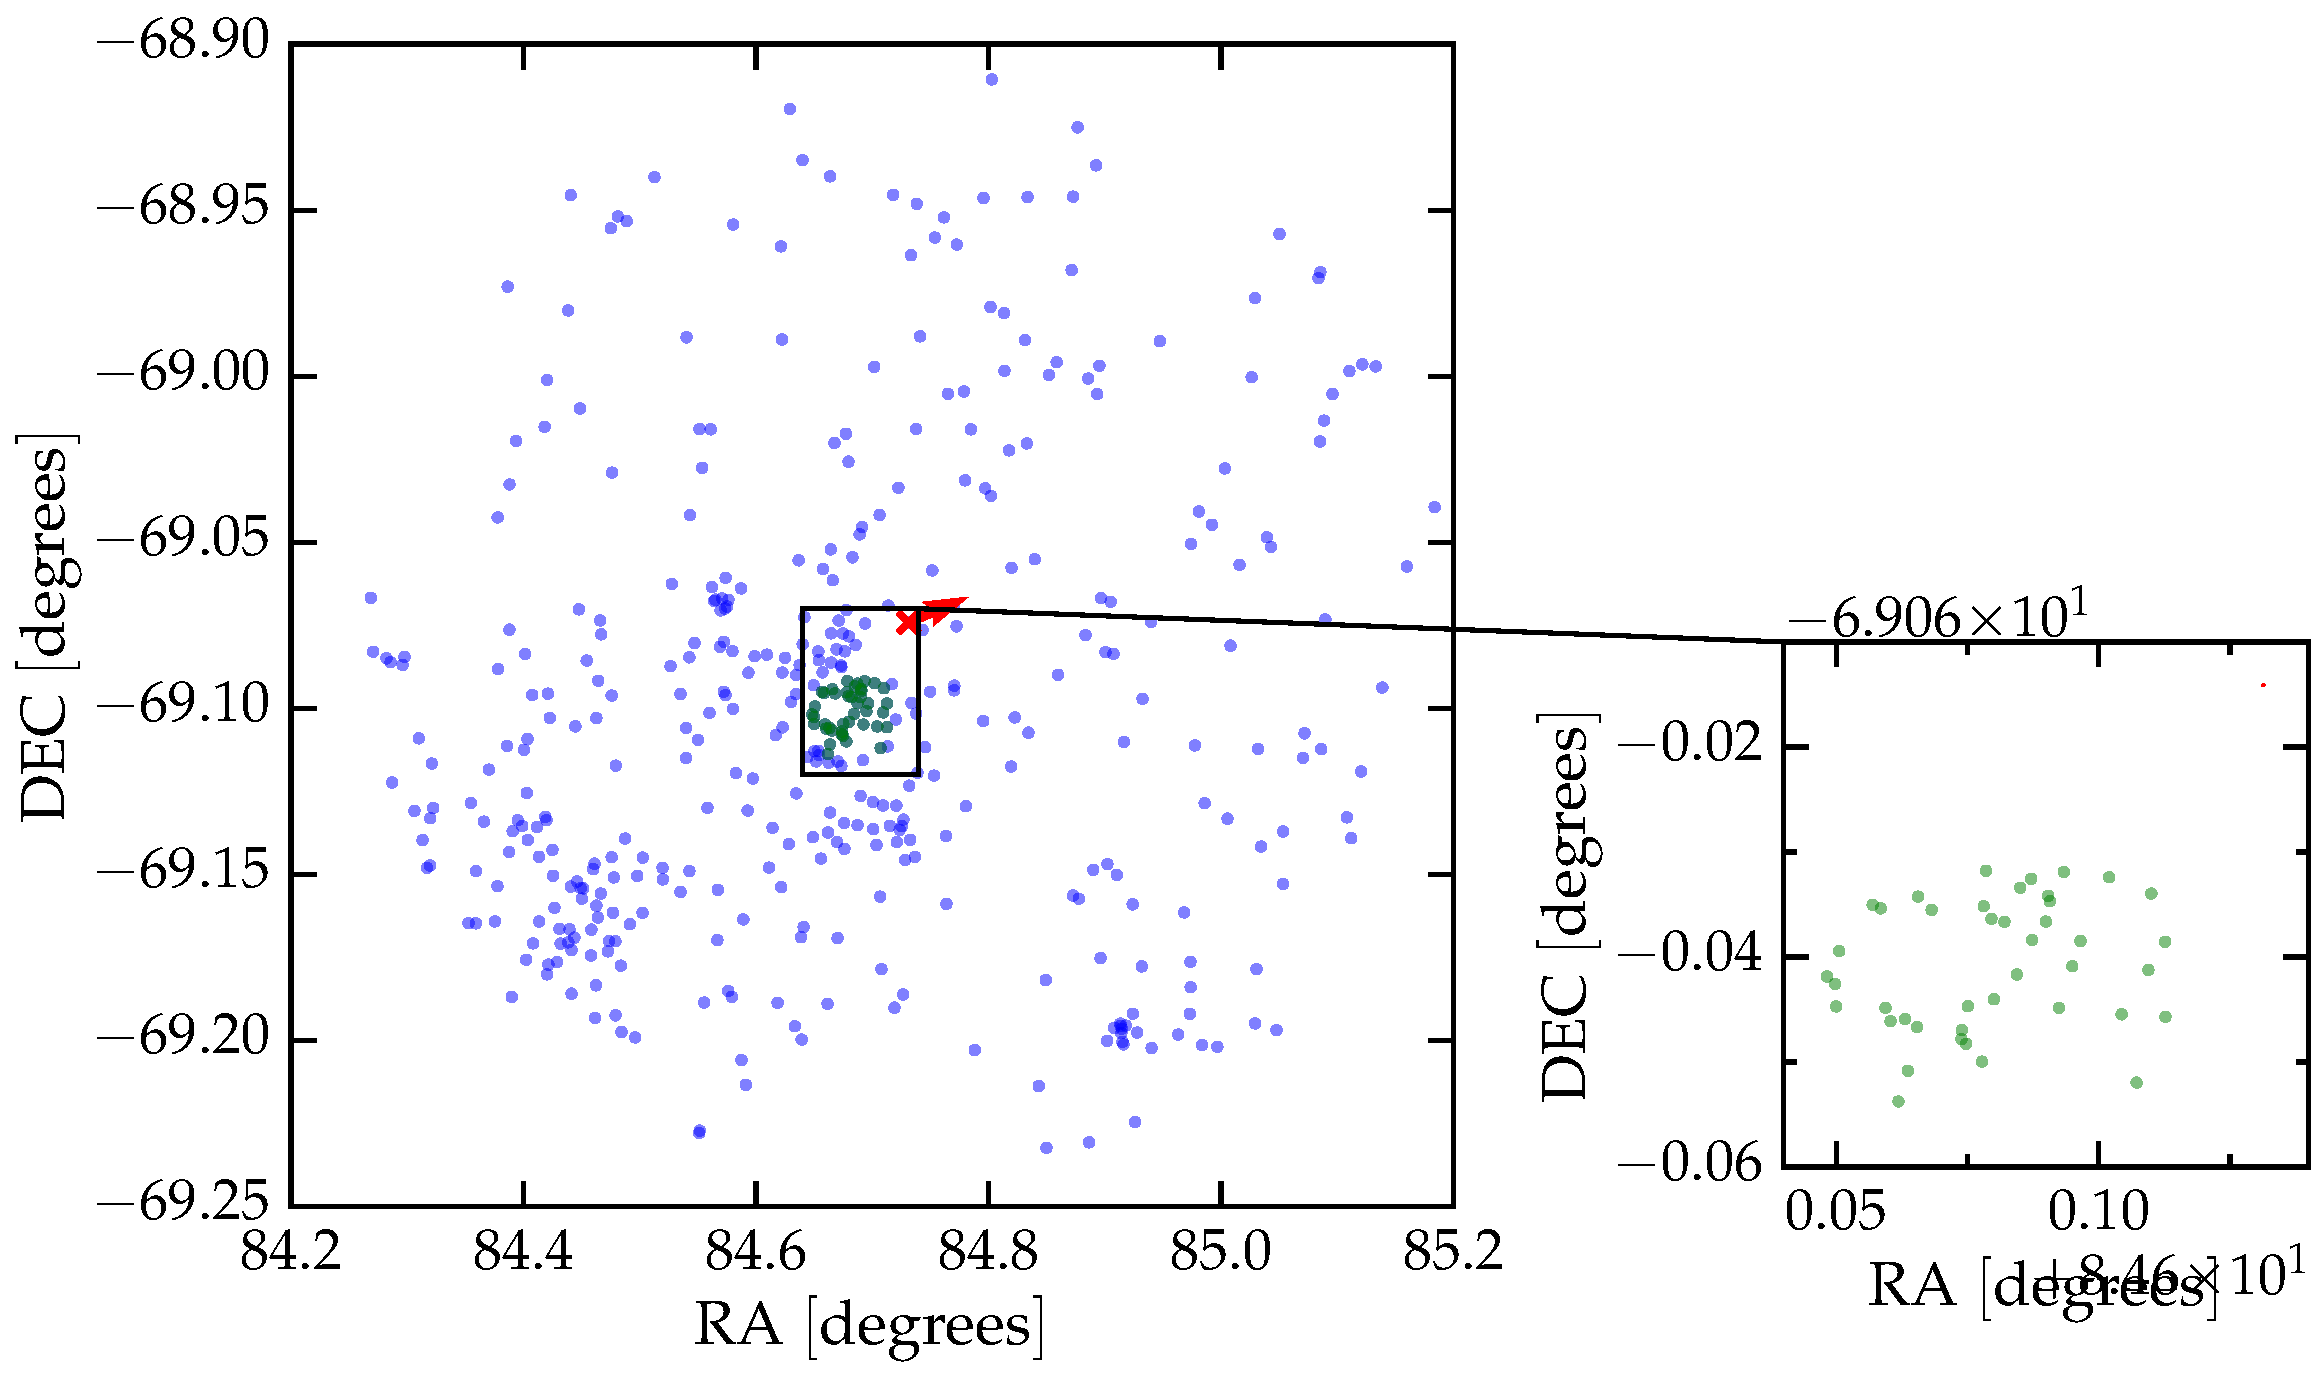
\includegraphics[width=\textwidth]{./figures/main_plot}  
  \caption{The red cross indicates the position of VFTS682. Blue stars
    are those we use to define the generic ``surroundings'', while the
    green dots indicate the stars we use to probe the core of R136,
    magnified in the inset. The red arrow shows the direction of the
    proper motion of VFTS682 relative to R136, and the gray shade
    indicates the uncertainty in the direction. \todo{orient properly, load  picture on background, add cone
      of uncertainty, maybe show pm for all stars in inset?}}
  \label{fig:main}
\end{figure*}

\section{Discussion}
\label{sec:discussion}

\todo{compare to Lennon: time of ejection is the same? what does it
  say for cluster}
\todo{say implications for center of R136 (same stars are there), how
  many ejected given this one, was a binary ejected in the other direction?}
\todo{does this imply there is a binary in the core ?}
\begin{itemize}
\item VFTS682 is a bona fide runaway with $v\sim60\,\mathrm{km\
    s^{-1}}$ thrown out from R136. Both its speed and the age of the
  cluster are consitent with a dynamical ejection.
  \item VFTS682 comes from R136 as was expected by
  \cite{bestenlehner:11, fujii:11, banerjee:12}, so it does not
  require isolated SFH to be explained
\item apparent age tension (connect to VFTS16 as well).
\item is R136 a single young cluster or a merger
\item estimate the influence of the gravitational potential of R136,
  what is its total mass and relaxation time?
\end{itemize}
\section{Summary}

1. Gaia data confirm a 150Msun runaway with v~60, thus the most
massive known to date
2. directions suggest ejection from R136, confirming prediction of
fuji+ banerjee+
2b. This fits with the observation from crowther of M>300Msun in R136
(and mention vfts682 has the same spectral type): the most likely
mechanism needs encounter with 2 more massive -> additional evidence
for Crowther claim
3. comment on final fate (BH)

Random notes: $v\sin(i)<200\,\mathrm{km\ s^{-1}}$ form \cite{schneider:18}, age $1.0\pm 0.2$\,Myr
from \cite{schneider:18}

Many other very massive stars are present in the surroundings this cluster, and a more
detailed analysis on the larger sample is desirable.


\bibliographystyle{aa}
\bibliography{bibliography/vfts682}

\begin{acknowledgements}
  The background image of \Figref{fig:main} is based on observations
  made with ESO Telescopes at the La Silla Observatory under programme
  ID 076.C-0888, processed and released by the ESO VOS/ADP group.
  This research made use of APLpy, an open-source plotting package for Python \cite{robitaille:12}.
  We are grateful to S.~Torres for extremely useful discussions on the
  Gaia DR2 dataset, and to M.~C.~Ramirez-Tannus for help with APLpy.
\end{acknowledgements}
\end{document}




%%% Local Variables:
%%% mode: latex
%%% TeX-master: t
%%% End:
